\documentclass{standalone}
\usepackage{tikz}
\usepackage{xcolor}
\usepackage{amsmath}
\usepackage{amssymb}
\usetikzlibrary{arrows.meta,positioning,decorations.pathreplacing,calc,bending}

% Colors
\definecolor{redtext}{RGB}{220,30,30}
\definecolor{bluetext}{RGB}{0,0,220}

% Font styles
\tikzset{
  redtitle/.style={font=\bfseries\small, text=redtext, align=center},
  bluetitle/.style={font=\bfseries\small, text=bluetext, align=center},
  label/.style={font=\small, align=center}
}

% Component styles
\tikzset{
  distribution/.style={thick, draw=black, smooth},
  arrow/.style={->, thick, bend left=20},
  redarrow/.style={->, thick, draw=redtext, bend left=30},
  bluearrow/.style={->, thick, draw=bluetext, bend right=40}
}

\begin{document}

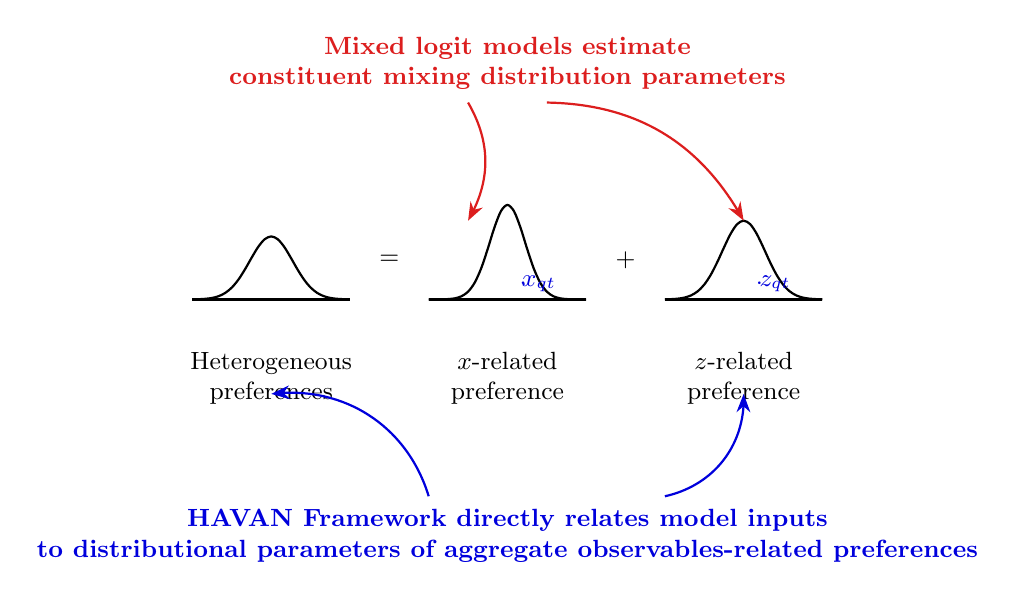
\begin{tikzpicture}[
  scale=1.0,
  every node/.style={font=\small},
  >=Stealth
]

  % Draw the distributions
  % Left distribution (heterogeneous preferences)
  \draw[distribution] (-4,0) -- (-2,0);
  \draw[distribution] plot[domain=-4:-2, smooth] (\x,{0.8*exp(-(\x+3)*(\x+3)/0.15)});
  \node[label] at (-3,-1) {Heterogeneous\\preferences};

  % Middle distribution (x-related preference)
  \draw[distribution] (-1,0) -- (1,0);
  \draw[distribution] plot[domain=-1:1, smooth] (\x,{1.2*exp(-(\x)*(\x)/0.1)});
  \node[label] at (0,-1) {$x$-related\\preference};

  % Right distribution (z-related preference)
  \draw[distribution] (2,0) -- (4,0);
  \draw[distribution] plot[domain=2:4, smooth] (\x,{1.0*exp(-(\x-3)*(\x-3)/0.15)});
  \node[label] at (3,-1) {$z$-related\\preference};

  % Equation symbols
  \node at (-1.5,0.5) {$=$};
  \node at (1.5,0.5) {$+$};

  % Variables
  \node[bluetext] at (0.2,0.2) {$\cdot$};
  \node[bluetext] at (0.4,0.2) {$x_{qt}$};
  \node[bluetext] at (3.2,0.2) {$\cdot$};
  \node[bluetext] at (3.4,0.2) {$z_{qt}$};

  % Red text and arrows
  \node[redtitle] at (0,3) {Mixed logit models estimate\\constituent mixing distribution parameters};
  \draw[redarrow] (-0.5,2.5) to (-0.5,1);
  \draw[redarrow] (0.5,2.5) to (3,1);

  % Blue text and arrows
  \node[bluetitle] at (0,-3) {HAVAN Framework directly relates model inputs\\to distributional parameters of aggregate observables-related preferences};
  \draw[bluearrow] (-1,-2.5) to (-3,-1.2);
  \draw[bluearrow] (2,-2.5) to (3,-1.2);

\end{tikzpicture}

\end{document}